\chapter[Validação e Avaliação da Ferramenta]{Validação, Avaliação da Ferramenta e Trabalhos Futuros}
\label{cap:cap4}

Nesse capítulo são apresentadas a metodologia utilizada para validação e avaliação de usabilidade da ferramenta e-TAPE, assim como a exposição e análise dos resultados obtidos
e a sugestão de trabalhos futuros. 

% 1a seção do capítulo 4
\section{Cenário da Avaliação}
\label{sec:cenario}
O objetivo desta avaliação foi validar a ferramenta desenvolvida com a utilização por possíveis usuários finais. Essa avaliação foi dividida em três etapas: 
obtenção das informações gerais dos usuários, realização de tarefas pré-determinadas e avaliação da usabilidade da ferramenta.

\par
Para a realização do experimento, foi disponibilizada uma máquina com a ferramenta e o questionário a ser respondido.
Na primeira etapa, os usuários participantes da avaliação foram informados quanto ao objetivo do experimento, orientados sobre os procedimentos a serem seguidos e questionados 
sobre as informações contidas na tabela \ref{tab:questionario}.

\begin{table}[!ht]
    \centering
    \caption{Primeira etapa do questionário aplicado aos participantes}
    \label{tab:questionario}
    \begin{tabular}{l*{2}{>{\raggedright\arraybackslash}p{0.2\linewidth}}}
    \toprule
        Pergunta        \\
    \midrule
        Qual seu sexo? \\
        Qual sua idade?\\
        Qual seu grau de escolaridade?\\
        Você conhece o conceito de participação eletrônica?\\
        Se respondeu sim na pergunta anterior,\\ por onde conheceu o conceito de participação eletrônica?\\
        Você costuma discutir questões sociais na internet?\\
        Se respondeu sim na pergunta anterior,\\ quando discutindo sobre questões sociais na internet,\\costuma discutir com: \\
        Você sabe o que é uma Taxonomia?\\
    \bottomrule
    \end{tabular}
\end{table}

\par
Após a primeira etapa, foi dado a cada usuário o tempo de cinco minutos para conhecer a taxonomia, lendo as definições dos grupos, classes e subclasses,
disponíveis na primeira página da aplicação. Após os cinco minutos, foi entregue a cada usuário duas descrições textuais sobre ferramentas de participação eletrônica.
A partir dessas descrições, cada usuário deveria classificar a ferramenta em questão de acordo com o que achasse mais adequado.
Essa abordagem foi adotada para que fosse possível a comparação entre a classificação de uma ferramenta de participação feita por um especialistas no assunto em comparação com
a mesma ferramenta de participação classificada por usuários leigos. O tempo gasto para leitura das descrições textuais e classificação das ferramentas foi cronometrado e registrado.
As descrições aplicadas aos respondentes podem ser encontradas no Apêndice deste trabalho.

\par
Na terceira etapa, após finalizada a interação do usuário com a ferramenta, o objetivo foi avaliar a usabilidade da ferramenta e-TAPE.
Para essa avaliação, foi utilizado o questionário \acrfull{sus}, desenvolvido por \citeonline{brooke1996sus}, composto de 10 itens \textit{likert}. 
Onde cada item corresponde a uma escala \textit{likert} de 5 pontos, sendo 1 atribuído a discordo totalmente, e 5 atribuído a concordo totalmente.

\begin{figure}[!ht]
    \centering
    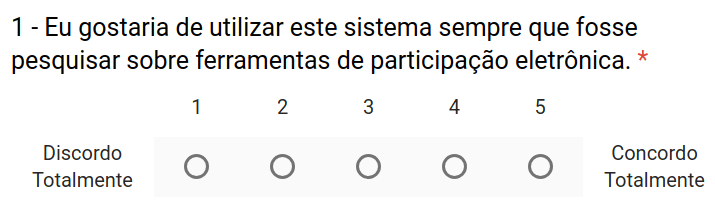
\includegraphics[scale=0.5]{./figuras/exemplo_pergunta.png}
    \caption{Exemplo de item \textit{Likert} presente no questionário}
    \label{fig:exemplo-pergunta}
\end{figure}

\par
Foi pedido aos respondentes, seguindo a metodologia de \citeonline{brooke1996sus}, para que logo após usar a aplicação, assinalasse sua resposta de maneira 
imediata ao término da leitura da descrição de cada item, evitando que se pensasse muito sobre a resposta. 
Todos os itens são de preenchimento obrigatório e caso o respondente não consiga responder a algum em particular, foi pedido que marcasse o ponto médio de valor 3.  

\par
Os dez itens presentes no questionário foram escolhidos, por \citeonline{brooke1996sus}, após a aplicação de um questionário com 50 itens em potencial, sobre dois sistemas diferentes. 
Desses 50 itens em potencial, foram selecionados os 5 com os maiores valores de concordância e os outros 5 com maiores valores de discordância. Assim, os esses 10 itens selecionados,
foram postos alternadamente, com o objetivo de evitar respostas automáticas, obrigando o respondente a se esforçar para pensar se concorda ou discorda de cada item. 

\par
O questionário \acrshort{sus}, permite o cálculo de um indicador para a usabilidade geral do sistema ao qual é aplicado, denominado como \textit{Score SUS} . 
\citeonline{brooke1996sus} definiu o cálculo do \textit{Score SUS} da seguinte forma:
Para os itens 1, 3, 5, 7 e 9, será o valor assinalado pelo respondente menos 1. Para os itens 2, 4, 6, 8 e 10, será 5 menos o valor assinalado. Após isso, a soma dos valores 
encontrados é multiplicada por 2,5, obtendo-se o \textit{Score SUS} para o questionário avaliado.

\par
Sendo assim, o questionário aplicado aos participantes deste trabalho, foi traduzido do questionário original e contextualizadas para a ferramenta e-TAPE,
pode ser encontrado Tabela \ref{tab:questionario3}

\begin{table}[!ht]
    \centering
    \caption{Segunda etapa do questionário aplicado aos participantes}
    \label{tab:questionario3}
    \begin{tabular}{l*{2}{>{\raggedright\arraybackslash}p{0.66\linewidth}}}
    \toprule
    Nº & Questão        \\
    \midrule
    1 & Eu gostaria de utilizar este sistema sempre que fosse pesquisar sobre ferramentas de participação eletrônica.\\
    2 & Eu achei a aplicação desnecessariamente complexa. \\
    3 & Eu achei a aplicação fácil de usar.\\
    4 & Eu acho que precisaria de apoio de um suporte técnico para ser possível interagir com essa aplicação.\\
    5 & Eu achei que as diversas funções nesta aplicação foram bem integradas. \\
    6 & Eu achei que houve muita inconsistência ou erros nesta aplicação. \\
    7 & Eu imaginaria que a maioria das pessoas, interessadas em ferramentas de participação eletrônica, aprenderia a usar essa aplicação rapidamente. \\
    8 & Eu achei a aplicação muito complicada. \\
    9 & Eu me senti muito confiante quanto às interações com essa aplicação. \\
    10 & Eu precisei aprender muitas coisas sobre ferramentas de participação eletrônica para que eu pudesse fazer uso da aplicação.\\
    \bottomrule
    \end{tabular}
\end{table}


\par
\citeonline{boucinha2013avaliaccao} mostram, que através das questões do \acrshort{sus}, também é possível identificar componentes de qualidade, indicados por \citeonline{nielsen199510},
da seguinte forma:

\begin{table}[!ht]
    \centering
    \caption{Componentes de qualidade, segundo \citeonline{nielsen199510}, por questões do \acrshort{sus}}
    \label{tab:componentesQualidadePorQuestao}
    \begin{tabular}{l*{2}{>{\raggedright\arraybackslash}p{0.2\linewidth}}}
    \toprule
        Componente de Qualidade & Questão(ões)        \\
    \midrule
        Facilidade de aprendizagem & 3, 4, 7 e 10 \\
        Eficiência & 5, 6 e 8 \\
        Facilidade de memorização & 2 \\
        Minimização dos erros & 6 \\
        Satisfação & 1, 4 e 9\\
    \bottomrule
    \end{tabular}
\end{table}

\par 
Onde segundo \citeonline{nielsen199510}, para avaliar cada componente de qualidade, deve-se fazer a média dos valores encontrados, durante o cálculo do \textit{Score SUS},
para o grupo de perguntas em questão.

\par
Os resultados encontrados, seguindo a metodologia de \citeonline{brooke1996sus}, juntamente com os componentes de qualidade identificados por \citeonline{nielsen199510},
são explanados na próxima seção.

\section{Resultados}
\label{sec:resultados}

O experimento contou com a participação de :X pessoas. Sendo ::X\% do sexo masculino e ::X\% do sexo feminino, como demostrado pelo gráfico presente
na Figura \ref{fig:grafico-sexo}. Além disso, é possíveis observar pela Figura \ref{fig:grafico-idade}, que a maioria dos participantes têm entre 20 e 25 anos de idade e 
estão com a graduação atualmente em curso, como explanado na Figura \ref{fig:grafico-grau}.

\begin{figure}[!ht]
    \centering
    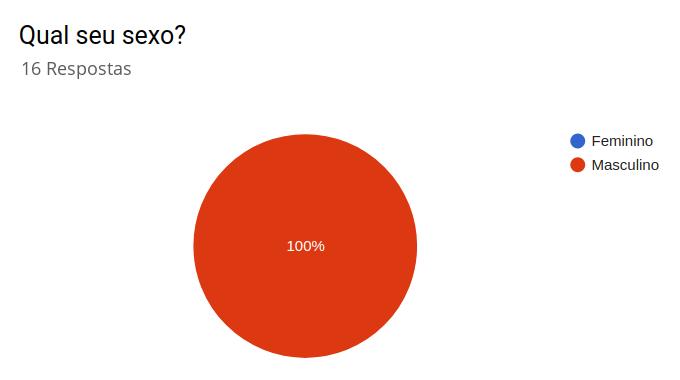
\includegraphics[scale=0.3]{./figuras/grafico_placeholder.png}
    \caption{Sexo dos participantes}
    \label{fig:grafico-sexo}
\end{figure}

\begin{figure}[!ht]
    \centering
    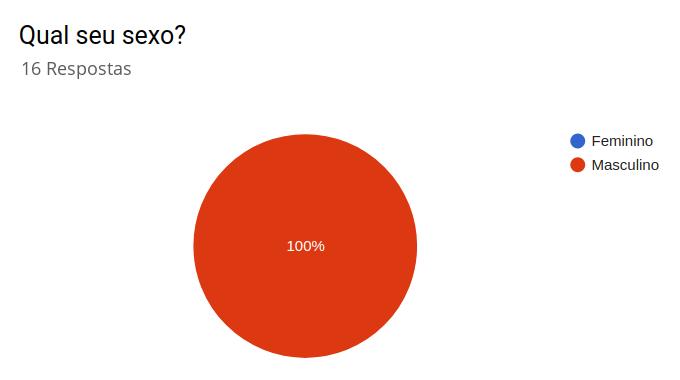
\includegraphics[scale=0.3]{./figuras/grafico_placeholder.png}
    \caption{Idade dos participantes}
    \label{fig:grafico-idade}
\end{figure}

\begin{figure}[!ht]
    \centering
    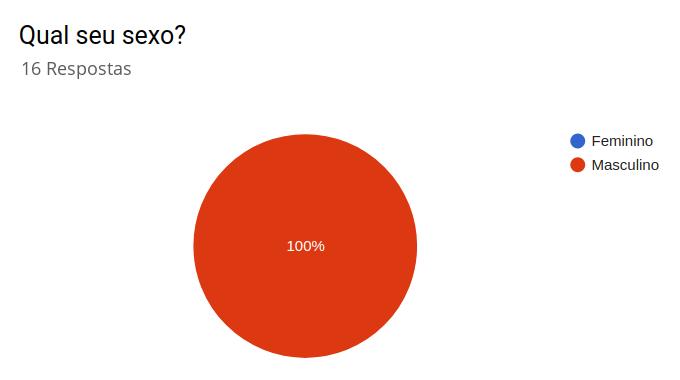
\includegraphics[scale=0.3]{./figuras/grafico_placeholder.png}
    \caption{Grau de escolaridade dos participantes}
    \label{fig:grafico-grau}
\end{figure}

%REVER COM MELISE
\par
Pôde-se perceber que a maioria das pessoas não conhecia o conceito de participação eletrônica, gráfico da Figura \ref{fig:grafico-participacao}. Porém grande parte dos participantes,
::X\%, respondeu que costuma discutir questões sociais na internet, desses ::X\% discutem com amigos, colegas e conhecidos, ::Y\% discutem com desconhecidos
e ::Y\% discutem com ambos os casos.

\par
Isso mostrou que questões sociais são importantes e os participantes gostam de discuti-las pela internet.
Esses dados estão representados pelos gráficos contidos nas Figuras \ref{fig:grafico-discu} e  \ref{fig:grafico-discu-alvo}, respectivamente. 

\begin{figure}[!ht]
    \centering
    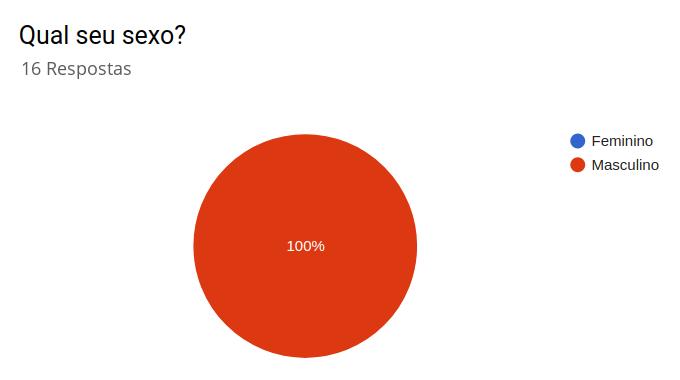
\includegraphics[scale=0.3]{./figuras/grafico_placeholder.png}
    \caption{Conhecimento sobre participação eletrônica dos participantes}
    \label{fig:grafico-participacao}
\end{figure}

\begin{figure}[!ht]
    \centering
    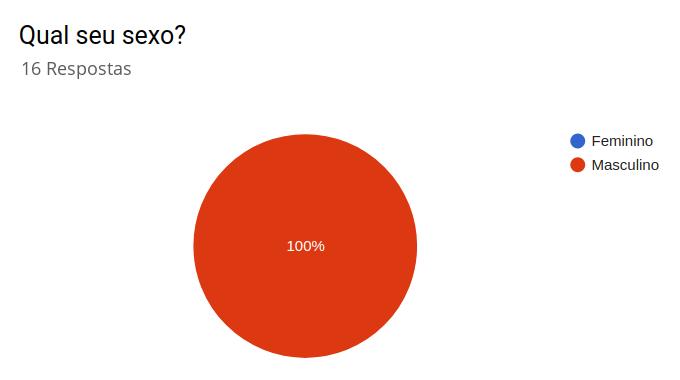
\includegraphics[scale=0.3]{./figuras/grafico_placeholder.png}
    \caption{Participantes que discutem questões sociais na internet}
    \label{fig:grafico-discu}
\end{figure}

\begin{figure}[!ht]
    \centering
    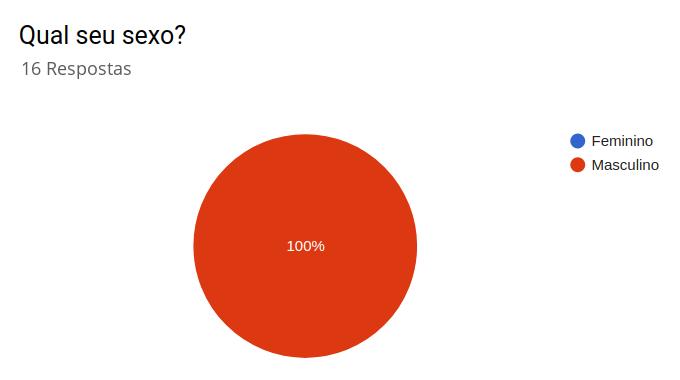
\includegraphics[scale=0.3]{./figuras/grafico_placeholder.png}
    \caption{Pessoas com as quais os participantes que discutem questões sociais na internet interagem.}
    \label{fig:grafico-discu-alvo}
\end{figure}

%REVER COM MELISE
\par
Quanto a última pergunta da primeira etapa, sobre o conhecimento prévio sobre Taxonomia, percebeu-se que a grande maioria ::X\%, não sabiam o que era uma Taxonomia, 
gráfico na Figura  \ref{fig:grafico-conhe-taxonomia}, mostrando que mesmo sendo um modelo de classificação antigo, não é conhecido por pessoas que não fazem utilização ou 
pesquisas sobre o assunto.

\begin{figure}[!ht]
    \centering
    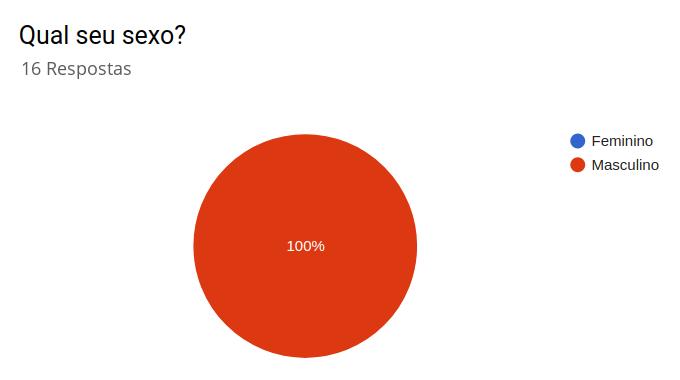
\includegraphics[scale=0.3]{./figuras/grafico_placeholder.png}
    \caption{Conhecimento do conceito de taxonomia pelos participantes.}
    \label{fig:grafico-conhe-taxonomia}
\end{figure}

\par
O tempo médio dos participantes para a conclusão da classificação das duas ferramentas solicitadas foi de X minutos e Y segundos, o gráfico na Figura \label{fig:grafico-tempo}
representa o tempo gasto por cada participante. Notou-se que participantes que tinham conhecimento prévio sobre ferramentas de participação e sobre taxonomia realizaram 
as tarefas em um tempo ::Z\% menor se comparado aos quais não tinham esse tipo de conhecimento.

\begin{figure}[!ht]
    \centering
    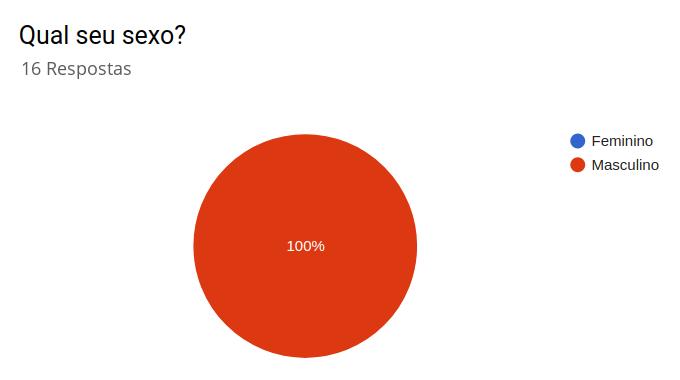
\includegraphics[scale=0.3]{./figuras/grafico_placeholder.png}
    \caption{Conhecimento do conceito de taxonomia pelos participantes.}
    \label{fig:grafico-tempo}
\end{figure}

\par 
O \textit{Score SUS} da aplicação e-TAPE foi de ::X, a Tabela \ref{tab:resultado-questionario} apresenta a média de pontuação de cada item do questionário \acrshort{sus}.
Como explicado na seção \ref{sec:cenario}, o \textit{Score Sus} dá-se pela soma dos resultados, multiplicada por 2,5.

\begin{table}[!ht]
    \centering
    \caption{\textit{Score SUS} de cada item do questionário aplicado}
    \label{tab:resultado-questionario}
    \begin{tabular}{l*{3}{>{\raggedright\arraybackslash}p{0.66\linewidth}p{0.1\linewidth}}}
    \toprule
    Nº & Questão & \textit{Score}    \\
    \midrule
    1 & Eu gostaria de utilizar este sistema sempre que fosse pesquisar sobre ferramentas de participação eletrônica. & ::X \\
    2 & Eu achei a aplicação desnecessariamente complexa. & ::X \\
    3 & Eu achei a aplicação fácil de usar. & ::X \\
    4 & Eu acho que precisaria de apoio de um suporte técnico para ser possível interagir com essa aplicação. & ::X \\
    5 & Eu achei que as diversas funções nesta aplicação foram bem integradas.  & ::X \\
    6 & Eu achei que houve muita inconsistência ou erros nesta aplicação.  & ::X \\
    7 & Eu imaginaria que a maioria das pessoas, interessadas em ferramentas de participação eletrônica, aprenderia a usar essa aplicação rapidamente. & ::X \\
    8 & Eu achei a aplicação muito complicada.  & ::X \\
    9 & Eu me senti muito confiante quanto às interações com essa aplicação.  & ::X \\
    10 & Eu precisei aprender muitas coisas sobre ferramentas de participação eletrônica para que eu pudesse fazer uso da aplicação. & ::X \\
    \bottomrule
    \end{tabular}
\end{table}

\par
A Tabela \ref{tab:resultado-componentes}, apresenta o resultado dos componentes de qualidade do \textit{software}. Sendo assim possível chegar a conclusão, pela metodologia aplicada, 
que a ferramenta e-TAPE satisfaz os critérios de qualidade propostos por \citeonline{nielsen199510}, de facilidade de aprendizagem (questões 3, 4, 7 e 10), eficiência (questões 5, 6 e 8),
facilidade de memorização (questão 2), minimização dos erros (questão 6) e satisfação (questões 1, 4 e 9).

\begin{table}[!ht]
    \centering
    \caption{Valor encontrado para cada componente de avaliação da qualidade da ferramenta e-TAPE}
    \label{tab:resultado-componentes}
    \begin{tabular}{l*{2}{>{\raggedright\arraybackslash}p{0.1\linewidth}}}
        \toprule
            Componente de Qualidade & Valor         \\
        \midrule
            Facilidade de aprendizagem & ::X \\
            Eficiência & ::X \\
            Facilidade de memorização & ::X \\
            Minimização dos erros & ::X \\
            Satisfação & ::X\\
        \bottomrule
        \end{tabular}
\end{table}

\section{Conclusão e Trabalhos Futuros}
\label{sec:conclusao}

